\documentclass[12pt]{article}
\usepackage{geometry}
\usepackage{amsfonts}
\usepackage{float}
\usepackage{amsmath}
\usepackage{tikz}
\usetikzlibrary{calc}

\geometry{
legalpaper, total={177.8mm, 290mm},left=6mm, right=6mm,
top=7mm, bottom=12mm,
}

\usepackage{letltxmacro}

\usepackage{setspace}

\begin{document}


\begin{center}
Mymensingh Girls' Cadet College \\
$3^{rd}$ Term Fornightly Examination - 2025 \\
Subject: Statistics-I \\
Class: XI \\
Marks: 20 \hfill Time: 40 Minutes
\end{center}



\hrule


\begin{center}
[\textbf{N.B.} – The figures of the right margin indicate full marks. Read 
the stems carefully and answer the associated questions. Answer all the questions.]\\
\end{center}

%\begin{center}
% \textbf{Group  - A}

%\end{center}
  \begin{enumerate}

 \item
  \textbf{A vehicle moves along the path ABCD, covering each segment at a uniform velocity.}

\begin{center}

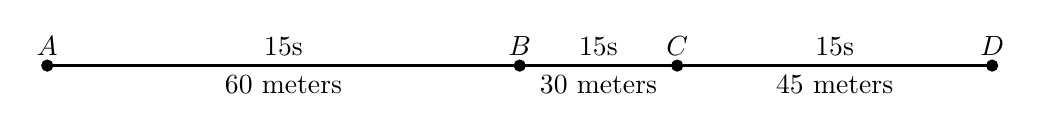
\begin{tikzpicture}
% Define the total length and segment lengths
\def\totalLength{12}
\def\segmentOne{6}   % 15s segment
\def\segmentTwo{2}   % 5s segment  
\def\segmentThree{4} % 10s segment

% Draw the main line
\draw[thick] (0,0) -- (\totalLength,0);

% Define the points
\coordinate (A) at (0,0);
\coordinate (B) at (\segmentOne,0);
\coordinate (C) at (\segmentOne+\segmentTwo,0);
\coordinate (D) at (\totalLength,0);

% Draw solid points at A, B, C, D
\foreach \point/\label in {A/A, B/B, C/C, D/D} {
    \filldraw[black] (\point) circle (2pt);
    \node[above] at (\point) {$\label$};
}

% Add time labels above the segments
\node[above] at ($(A)!0.5!(B)$) {15s};
\node[above] at ($(B)!0.5!(C)$) {15s};
\node[above] at ($(C)!0.5!(D)$) {15s};

% Optional: Add distance markers below the line
\node[below] at ($(A)!0.5!(B)$) {60 meters};
\node[below] at ($(B)!0.5!(C)$) {30 meters};
\node[below] at ($(C)!0.5!(D)$) {45 meters};


\end{tikzpicture}
  \end{center}
  \begin{enumerate}
    \item
	What is the formula of harmonic mean? \hfill 1
    \item
	When should we use the harmonic mean? \hfill 2
    \item  
	Find the average velocity of the vehicle. \hfill 3
    \item
	Compare the average speed estimated using the arithmetic and harmonic mean and \\ verify their suitability in the given situation. \hfill 4
  \end{enumerate}

\end{enumerate}
\begin{center}
--- AAM ---
\end{center}
  \vspace{1cm}
  


\end{document}